
%%%%%%%%%%%%%%%%%%%%%%%%%%%%%%%%%%%%%%%%%%%%%%%%%%%%%%%%%%%%%%%%%%%%%%%%%%%%%%%%
%
% Gadget2
%
%%%%%%%%%%%%%%%%%%%%%%%%%%%%%%%%%%%%%%%%%%%%%%%%%%%%%%%%%%%%%%%%%%%%%%%%%%%%%%%%

\section{Simulations with \gadgettwo}
\label{sec:gadget}

%%%%%%%%%%%%%%%%%%%%%%%%%%%%%%%%%%%%%%%%%%%%%%%%%%%%%%%%%%%%%%%%%%%%%%%%%%%%%%%%


We use the massively parallel TreeSPH cosmological \nbody\ simulation code \gadgettwo\ for the dark matter simulations presented in this work.  In this section, we begin with a discussion of the fundamental concepts presented in the original \gadget\ code, then proceed to the improvements made in the \gadgettwo\ code.




%~~~~~~~~~~~~~~~~~~~~~~~~~~~~~~~~~~~~~~~~~~~~~~~~~~~~~~~~~~~~~~~~~~~~~~~~~~~~~~~
\subsection{Fundamentals of \gadget}
\label{subsec:gadget--gadget}
%~~~~~~~~~~~~~~~~~~~~~~~~~~~~~~~~~~~~~~~~~~~~~~~~~~~~~~~~~~~~~~~~~~~~~~~~~~~~~~~


Text goes here.



%:::::::::::::::::::::::::::::::::::::::::::::::::::::::::::::::::::::::::::::::
\subsubsection{Force Calculation and Softening}
\label{subsubsec:gadget--gadget--softening}
%:::::::::::::::::::::::::::::::::::::::::::::::::::::::::::::::::::::::::::::::


Text goes here.

\begin{figure}[t]
	\centering
	\begin{subfigure}{}
		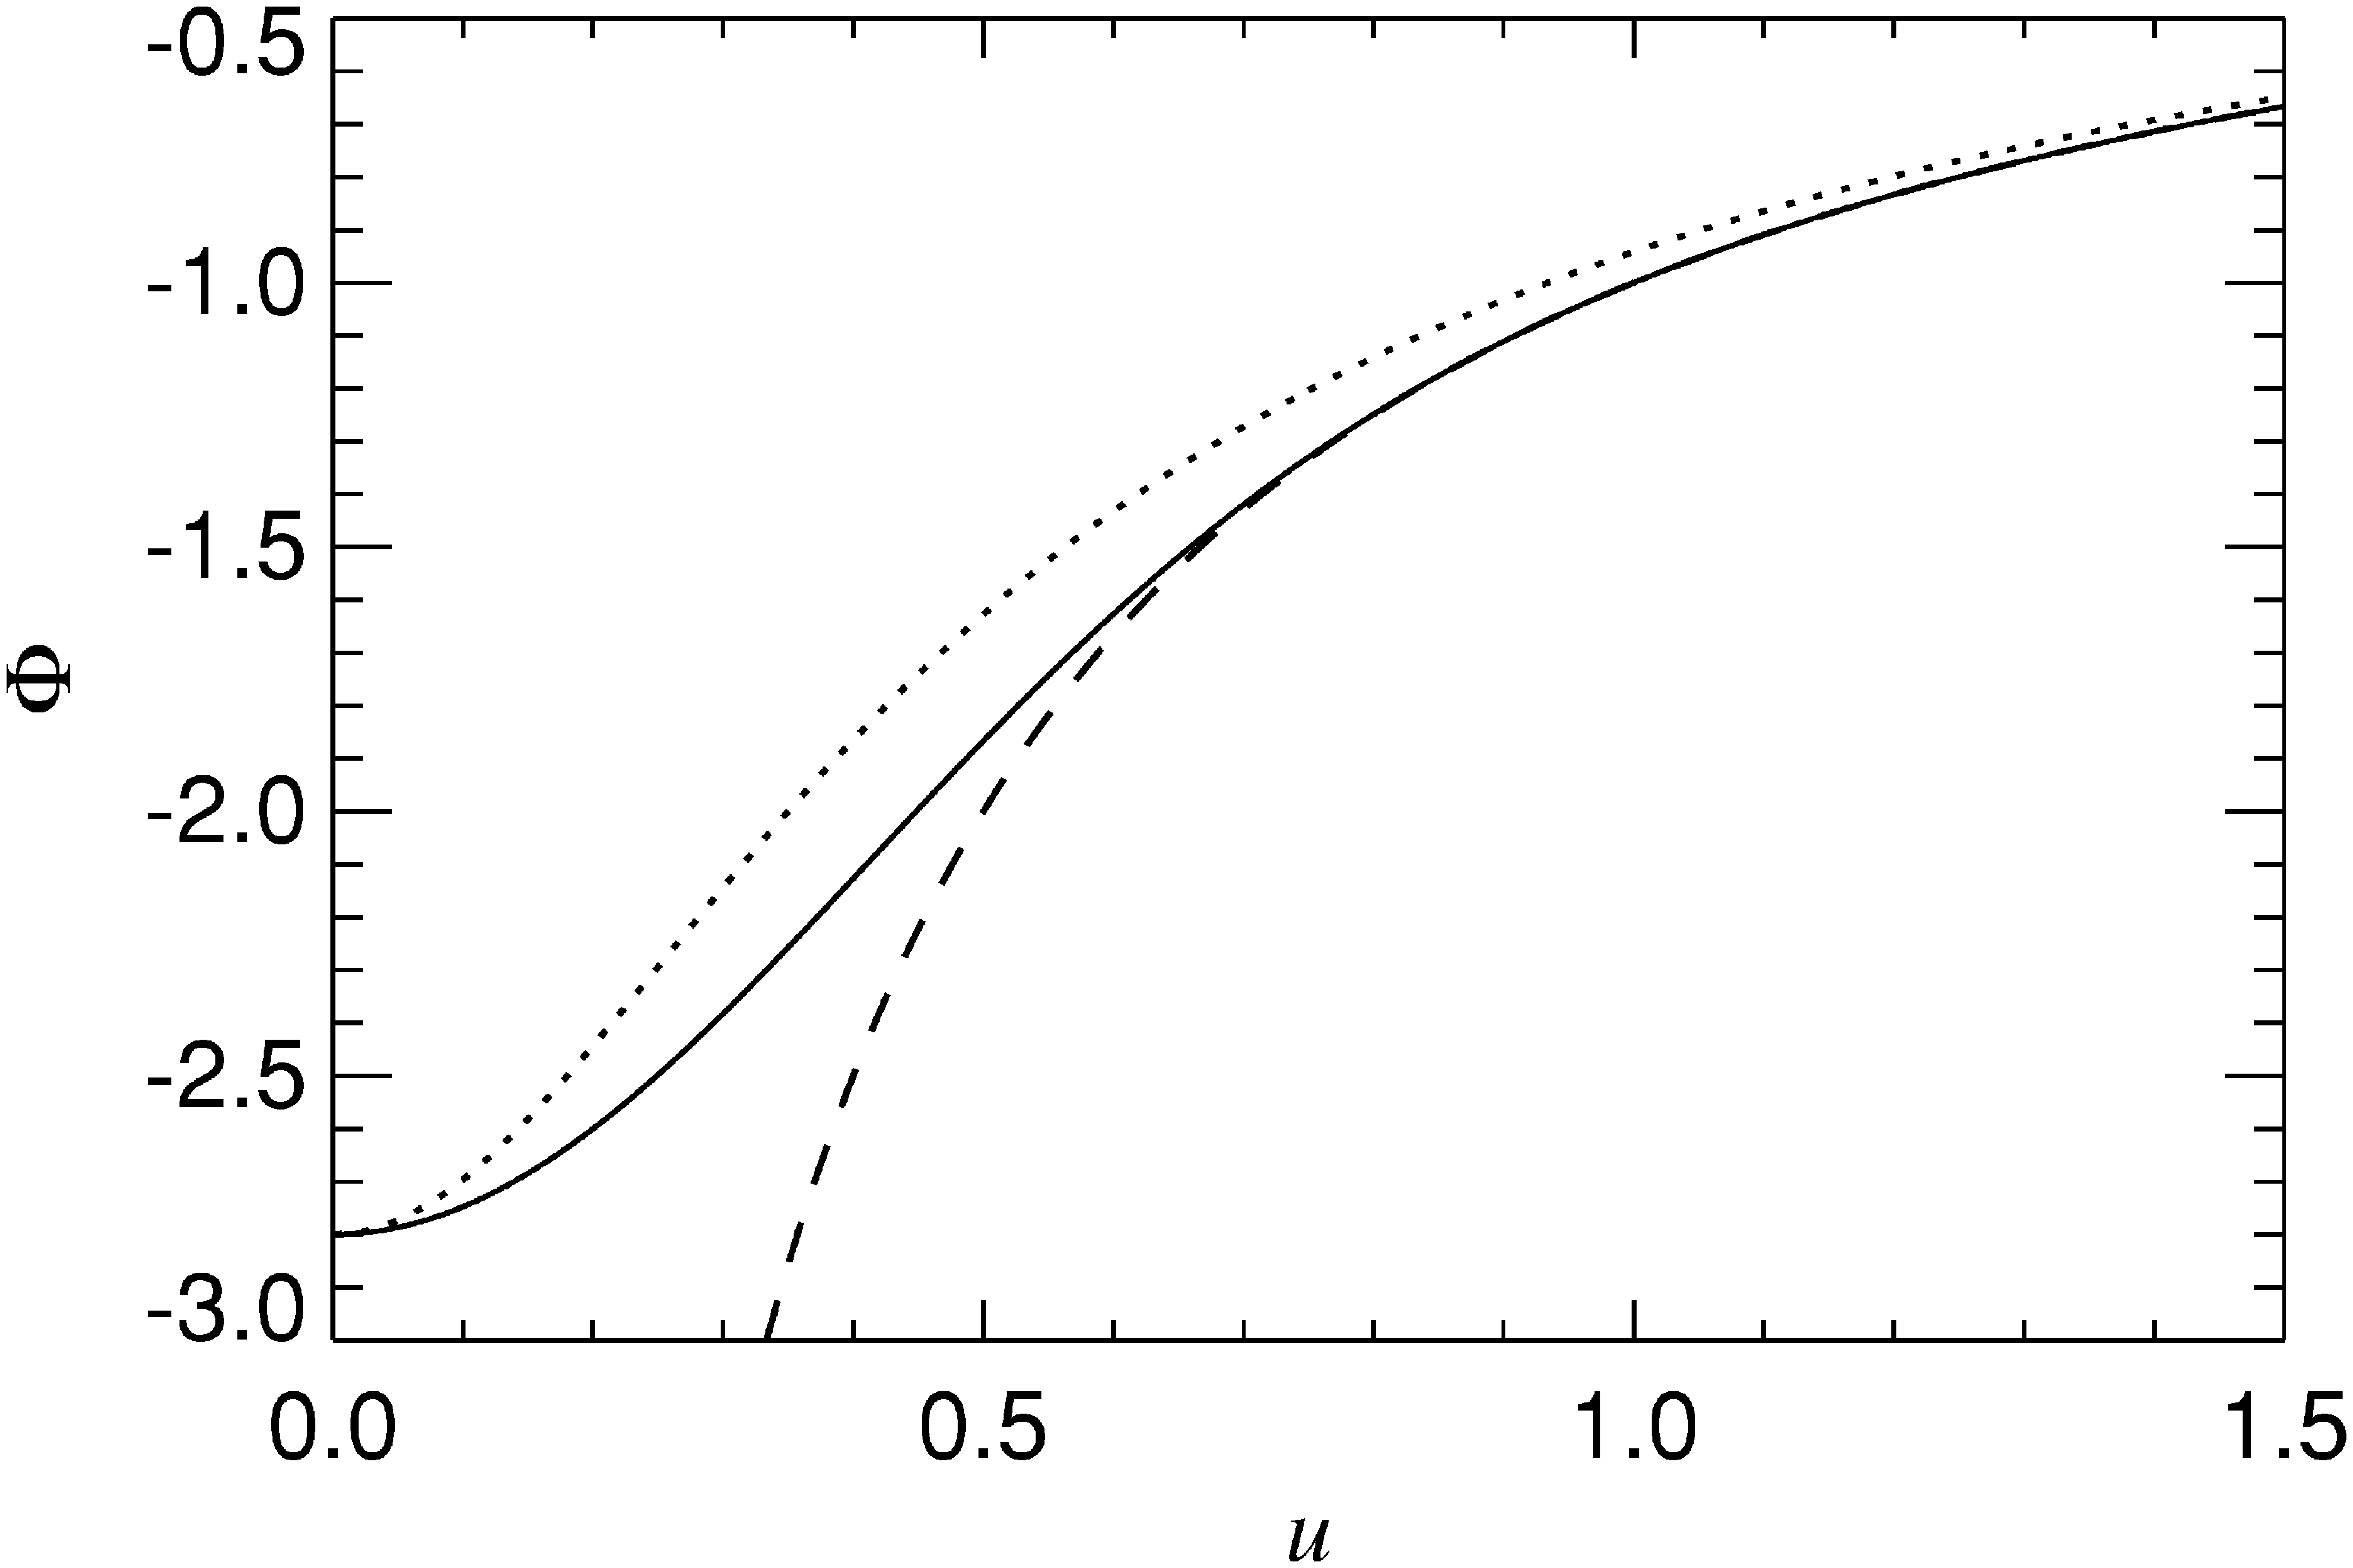
\includegraphics[width=0.45\linewidth]{gadget/softened_potential.eps}
	\end{subfigure}
	~
	\begin{subfigure}{}
		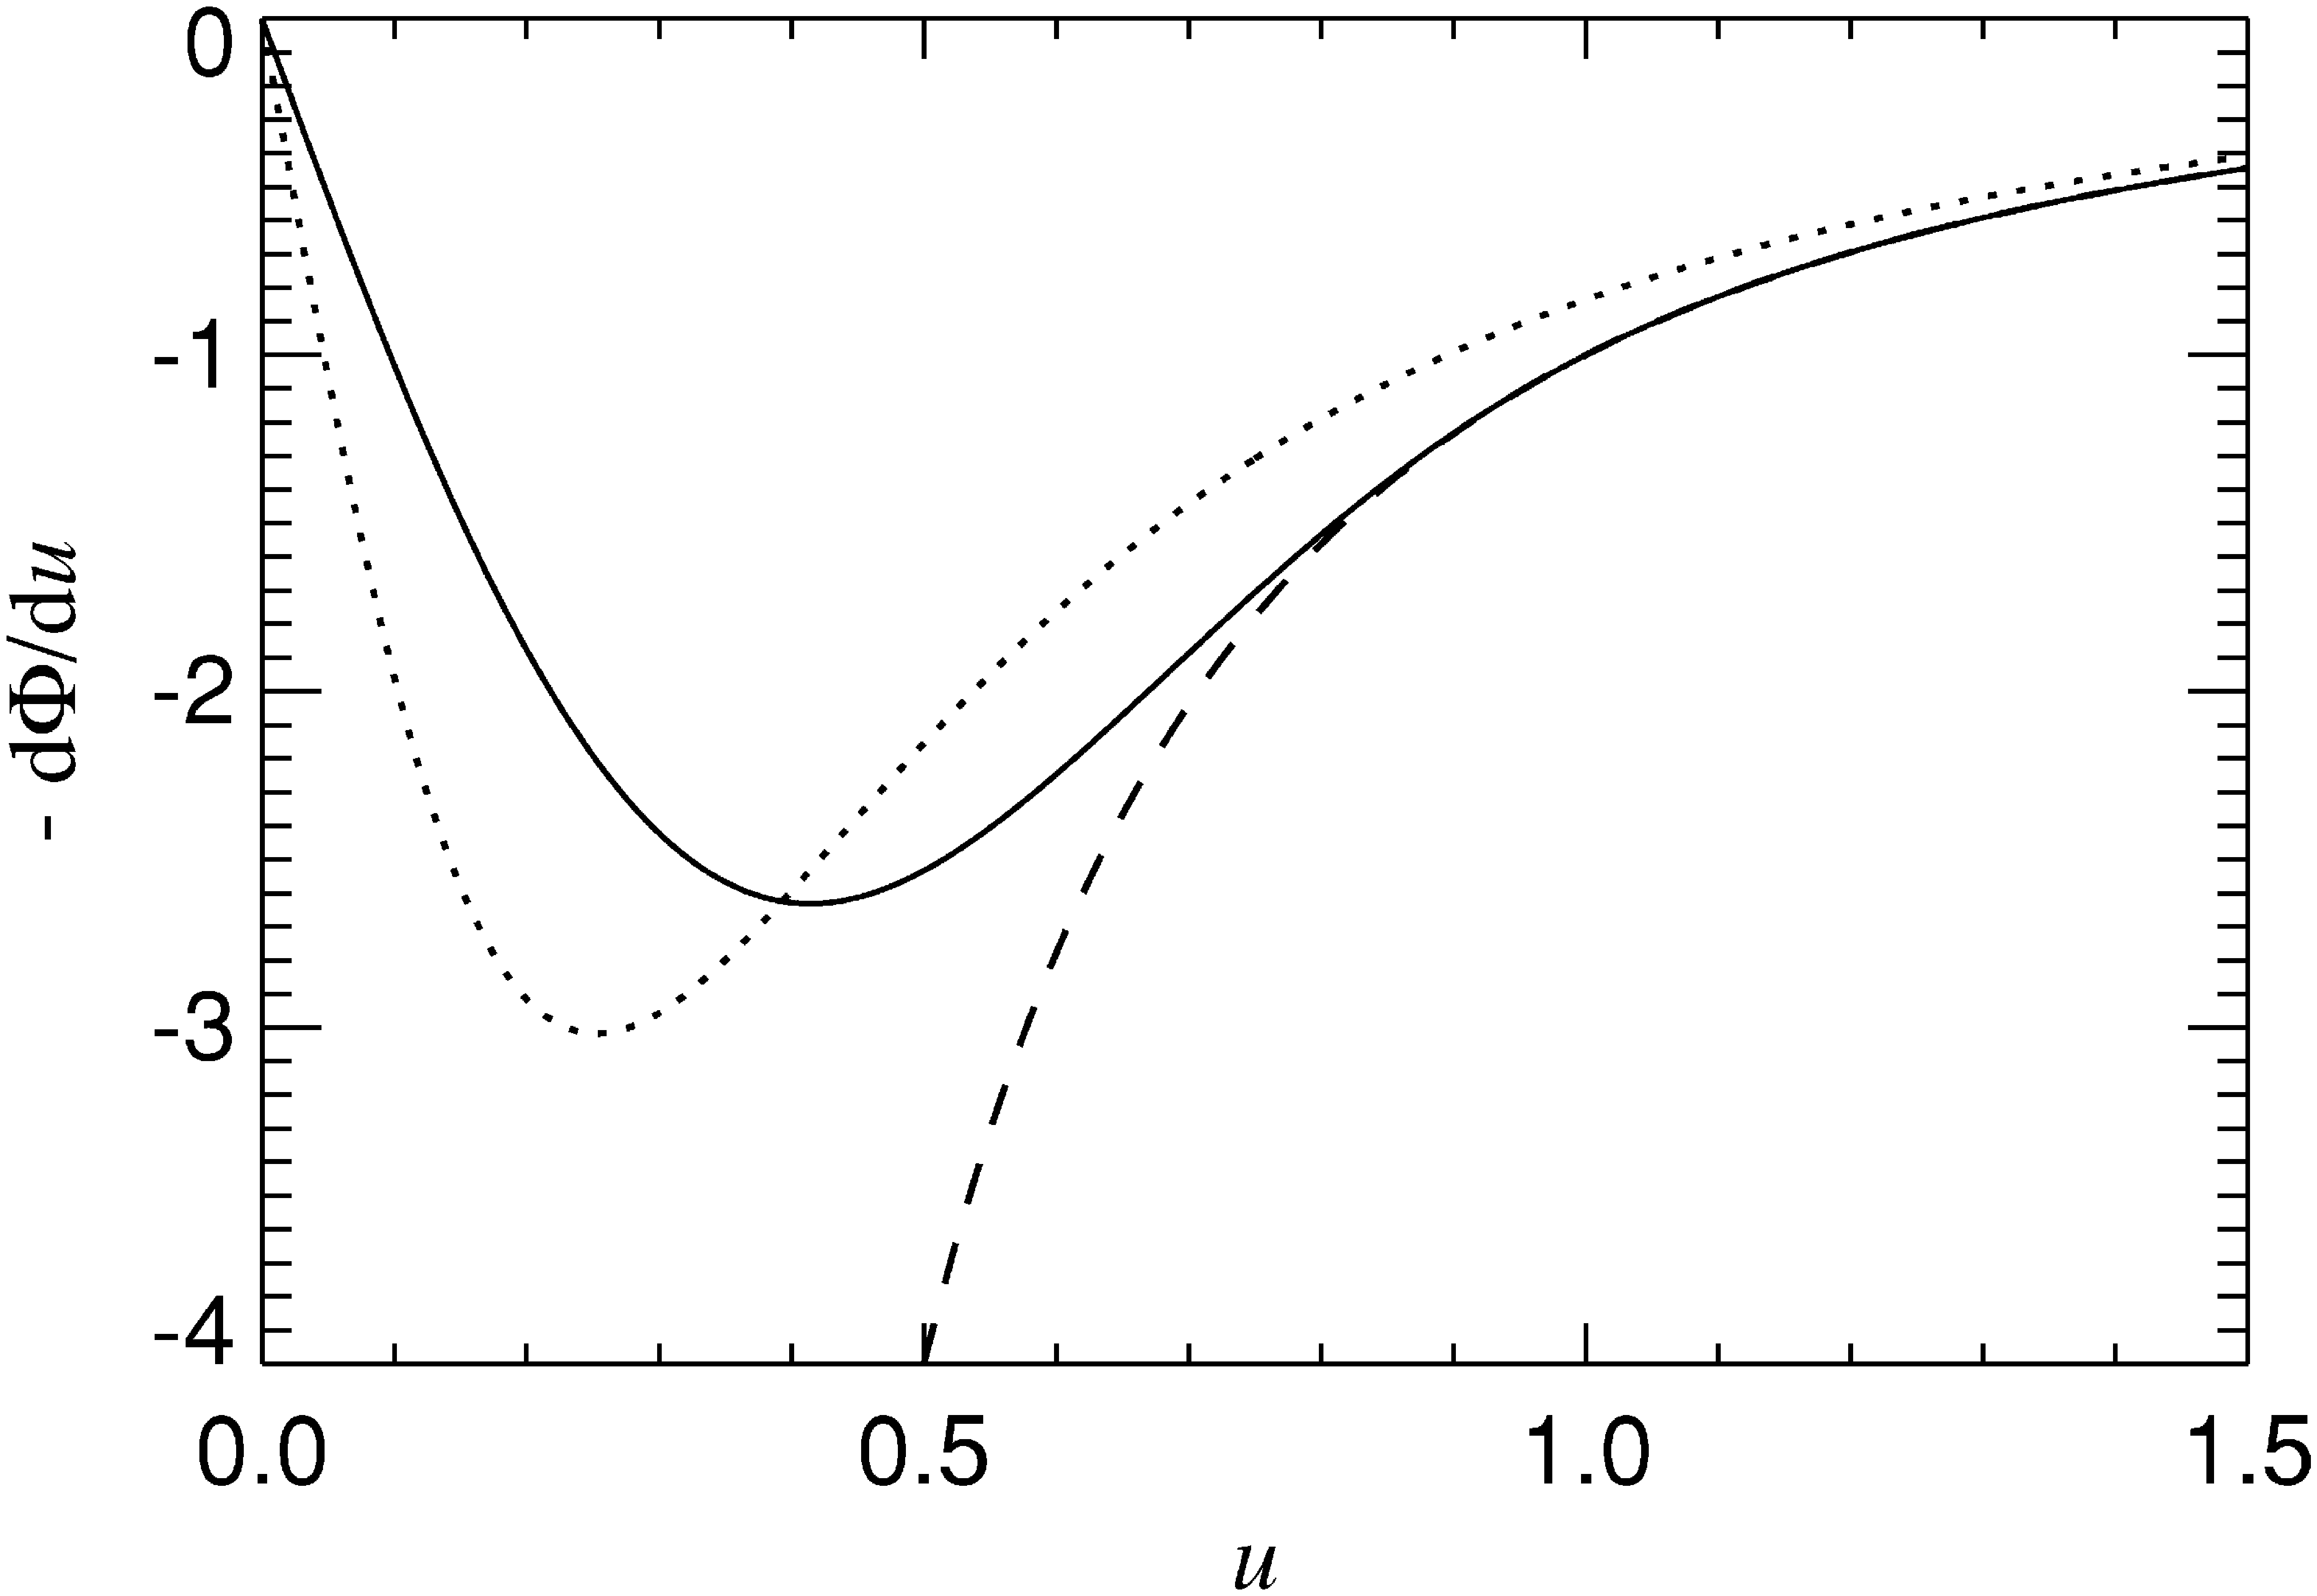
\includegraphics[width=0.45\linewidth]{gadget/softened_force.eps}
	\end{subfigure}
	\caption[Potential and force softening.]{Potential (\emph{left}) and force (\emph{right}) softening.}
	\label{fig:gadget--softening}
\end{figure}



%:::::::::::::::::::::::::::::::::::::::::::::::::::::::::::::::::::::::::::::::
\subsubsection{Trees}
\label{subsubsec:gadget--gadget--trees}
%:::::::::::::::::::::::::::::::::::::::::::::::::::::::::::::::::::::::::::::::


Text goes here.

\begin{figure}[t]
	\centering
	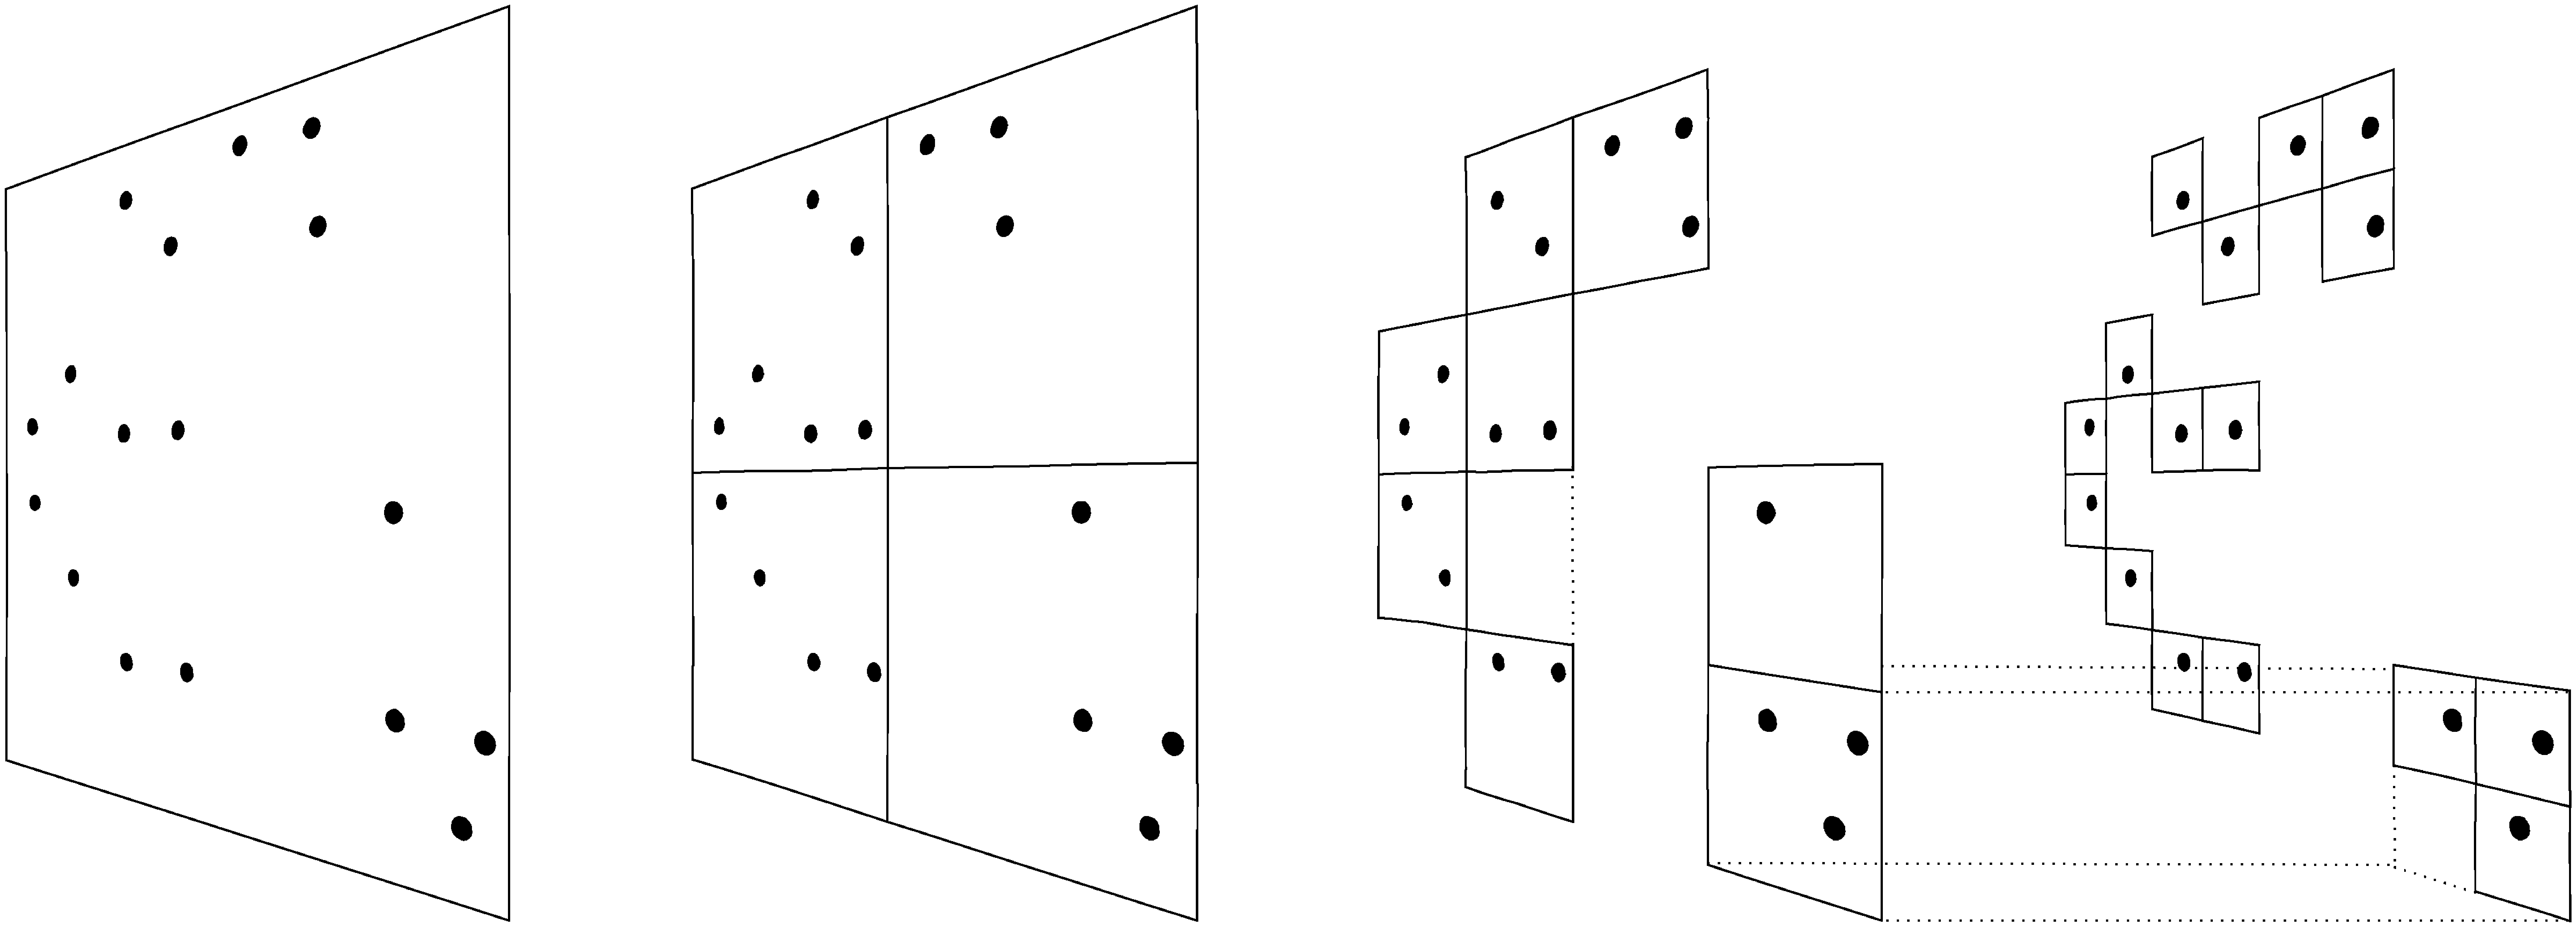
\includegraphics[width=\linewidth]{gadget/tree.eps}
	\caption[Barns-Hut oct-tree in two dimensions.]{Barns-Hut oct-tree in two dimensions.}
	\label{fig:gadget--tree}
\end{figure}



%:::::::::::::::::::::::::::::::::::::::::::::::::::::::::::::::::::::::::::::::
\subsubsection{Parallelization}
\label{subsubsec:gadget--gadget--parallelization}
%:::::::::::::::::::::::::::::::::::::::::::::::::::::::::::::::::::::::::::::::


Text goes here.

\begin{figure}[t]
	\centering
	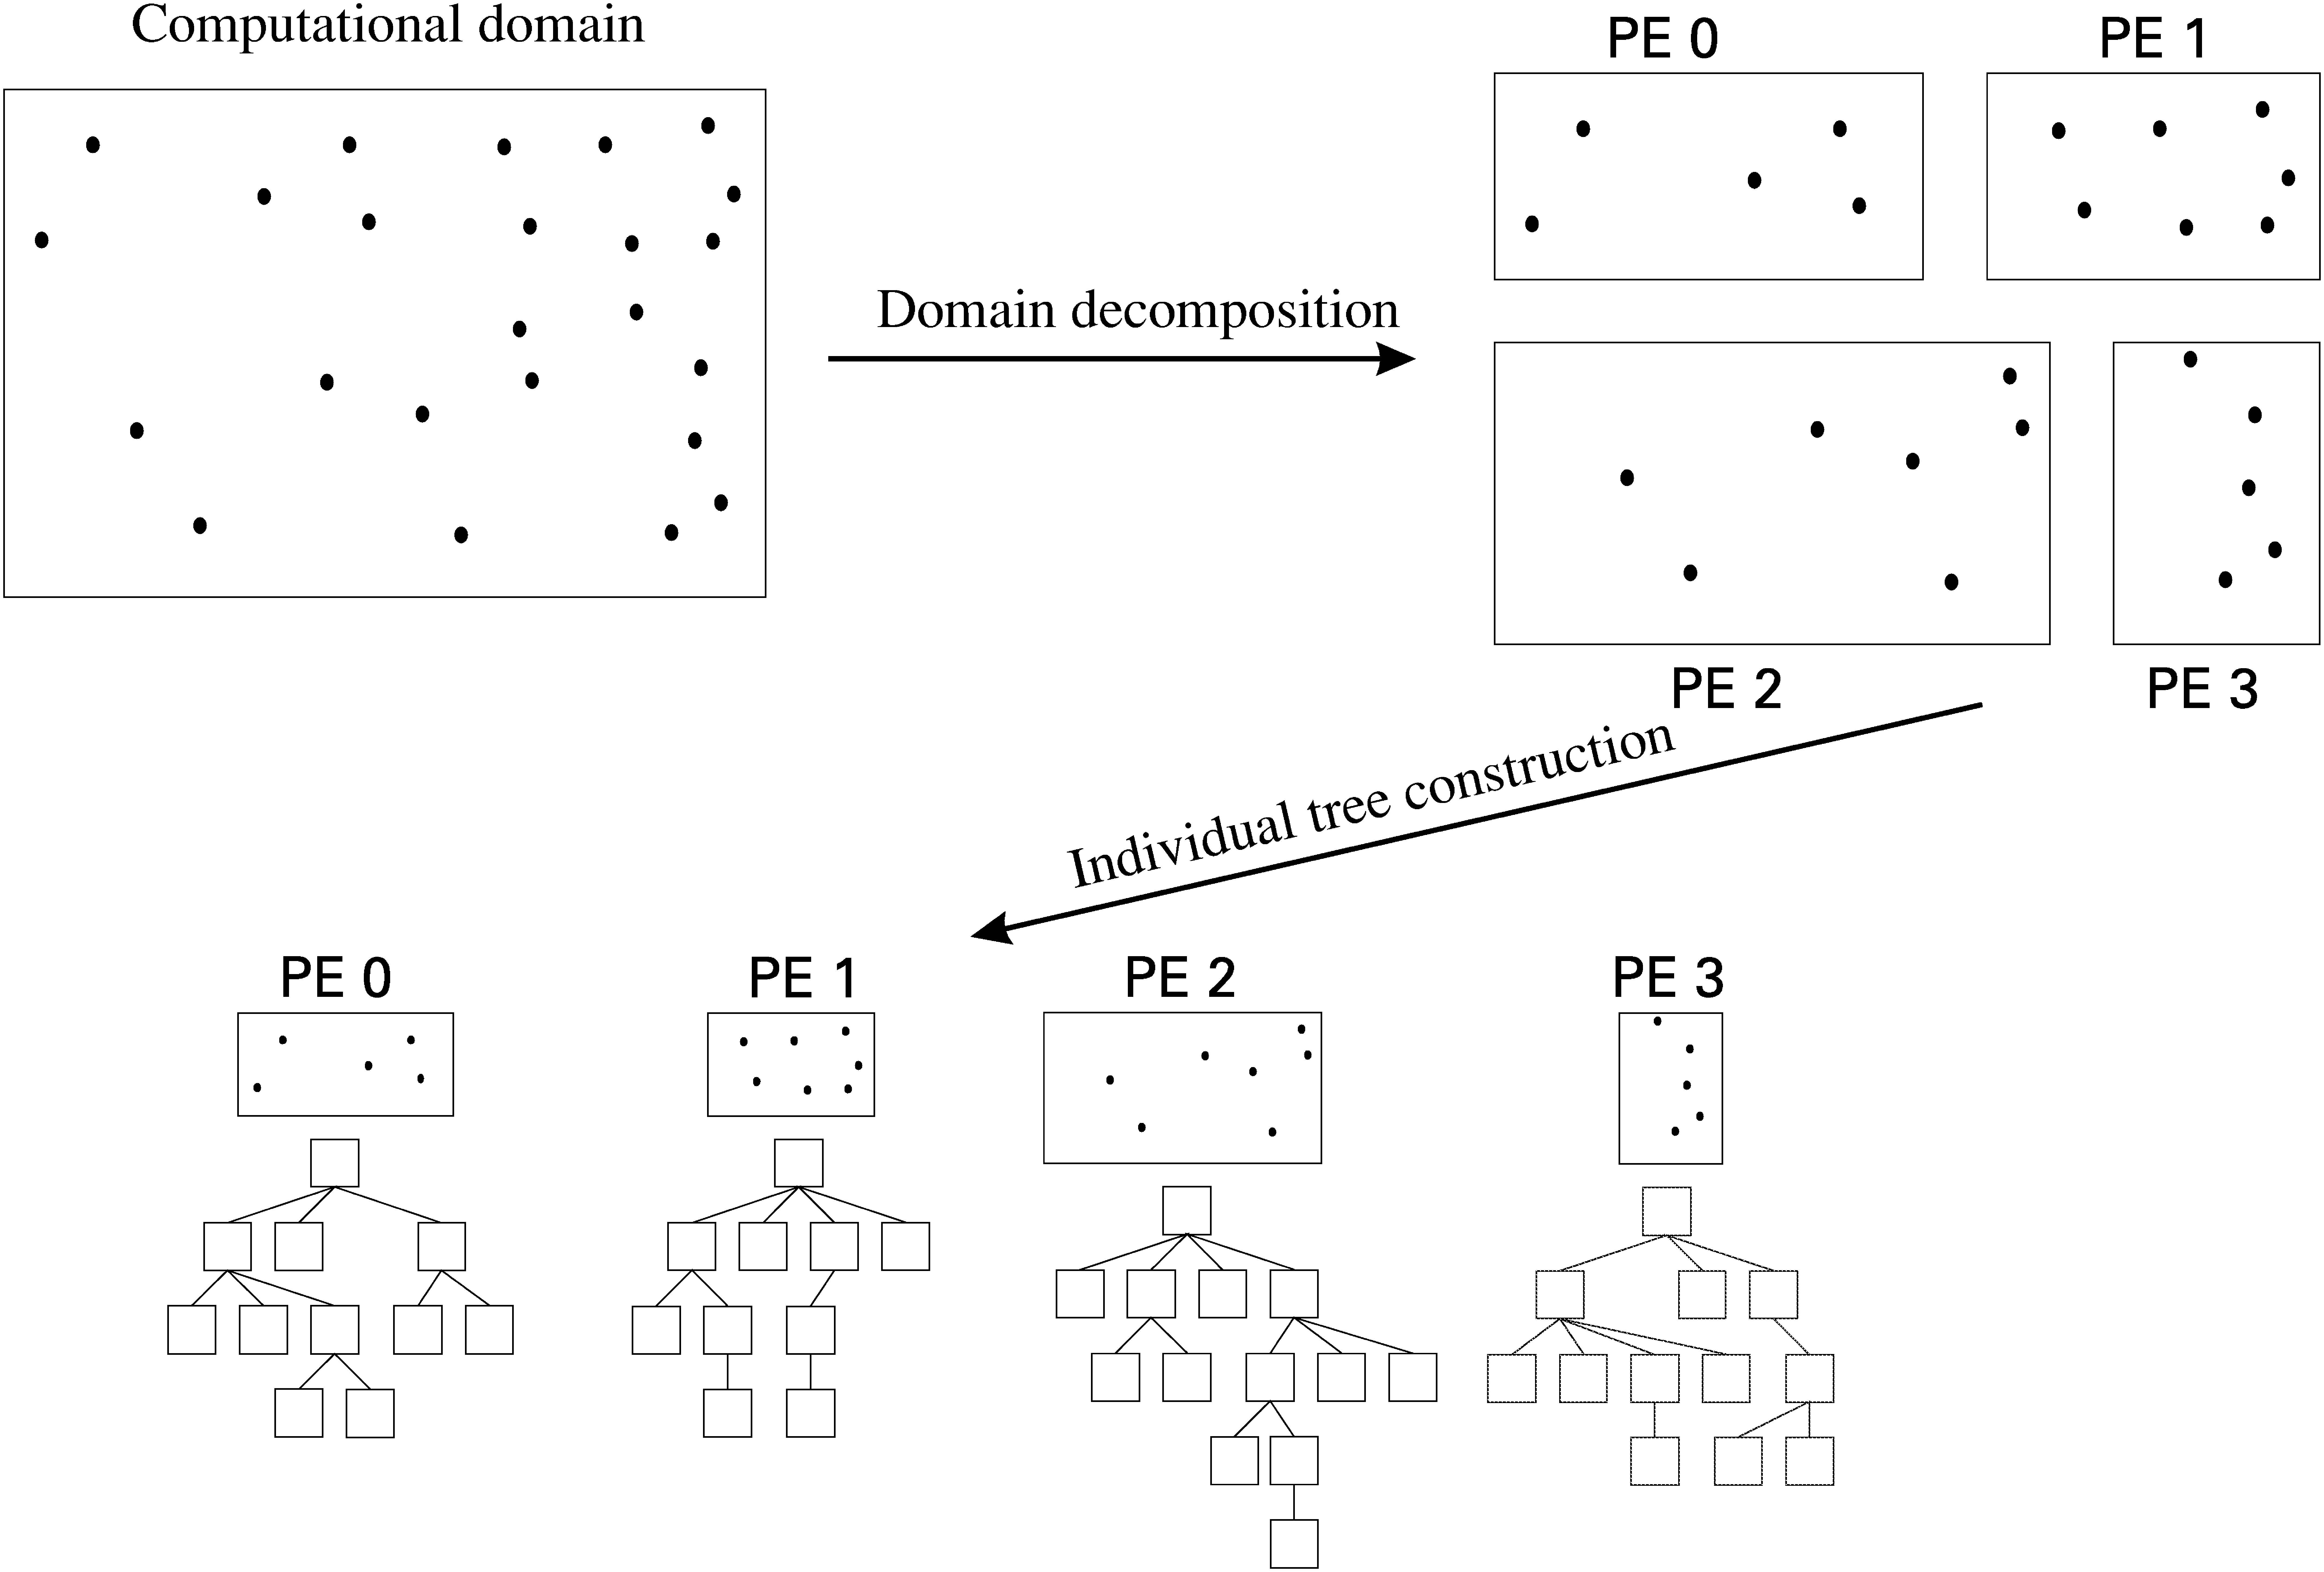
\includegraphics[width=\linewidth]{gadget/domain_decomp.eps}
	\caption[Domain decomposition.]{Domain decomposition.}
	\label{fig:gadget--domain_decomp}
\end{figure}

\begin{figure}[t]
	\centering
	
\includegraphics[width=\linewidth]{gadget/force_parallelism.eps}
	\caption[Force parallelism.]{Force parallelism.}
	\label{fig:gadget--force_parallelism}
\end{figure}



%:::::::::::::::::::::::::::::::::::::::::::::::::::::::::::::::::::::::::::::::
\subsubsection{Metrics}
\label{subsubsec:gadget--gadget--metrics}
%:::::::::::::::::::::::::::::::::::::::::::::::::::::::::::::::::::::::::::::::


Text goes here.

\begin{figure}[t]
	\centering
	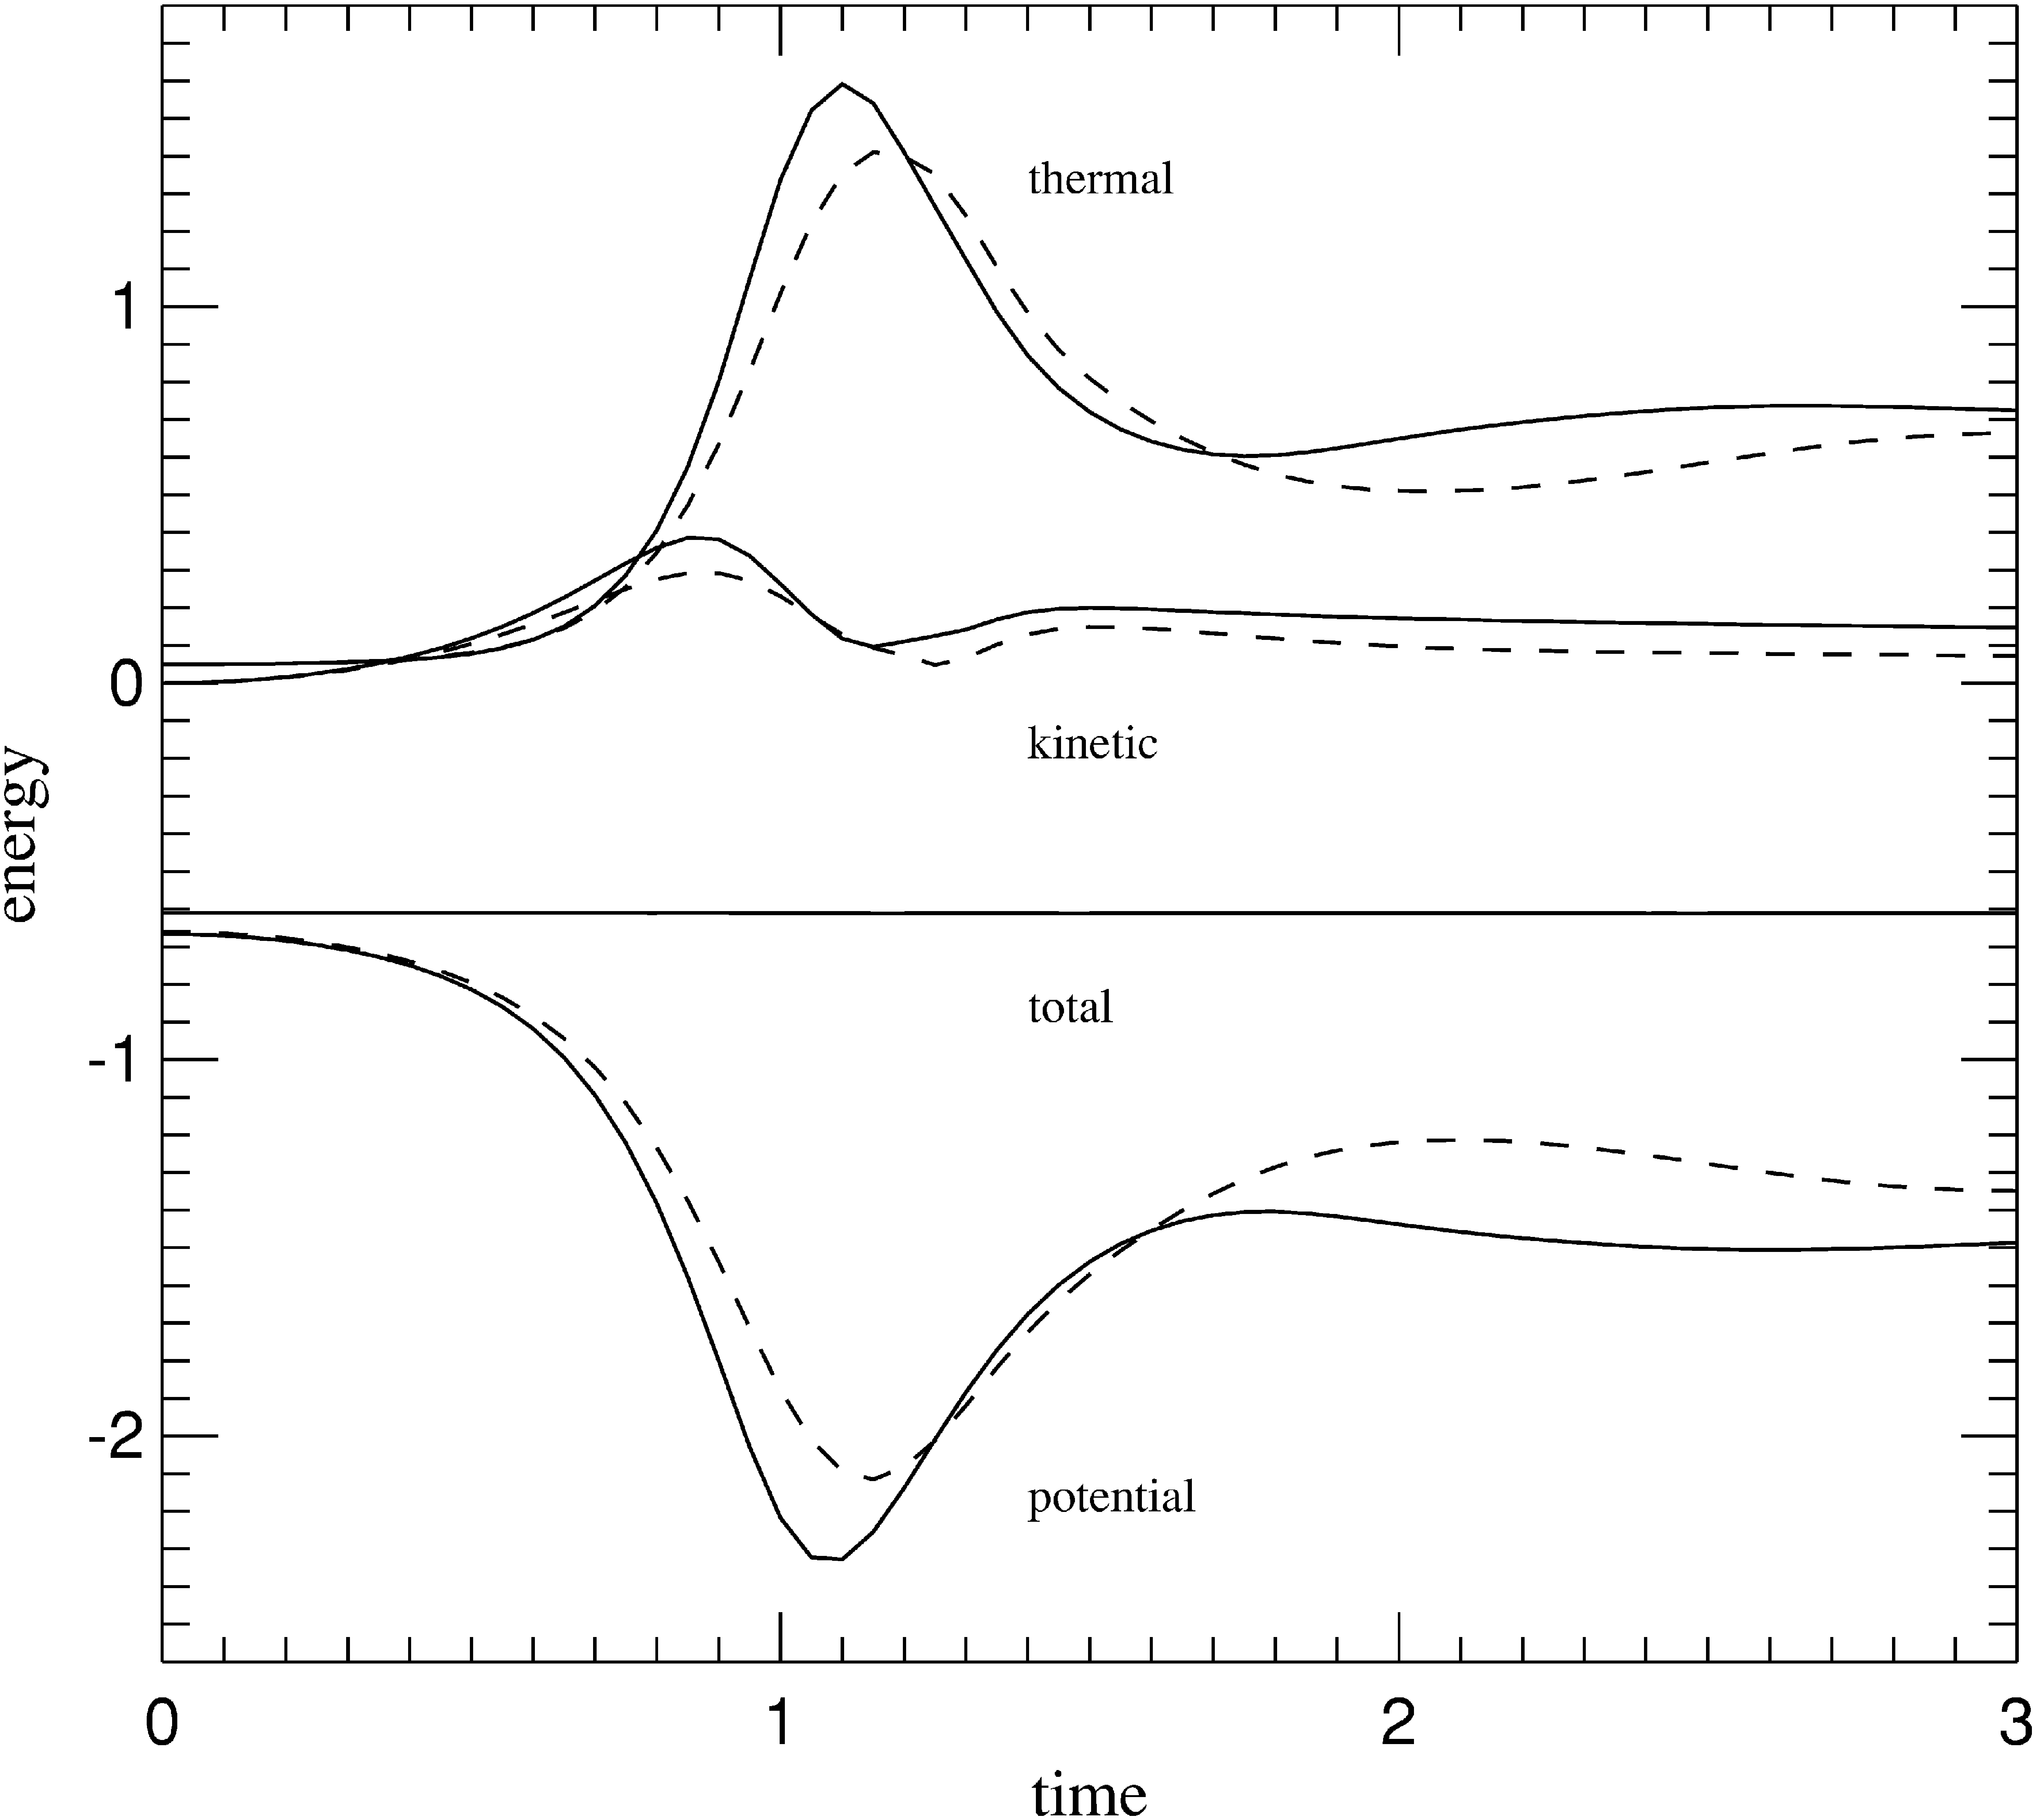
\includegraphics[width=0.75\linewidth]{gadget/energy_conservation.eps}
	\caption[Energy conservation for an initially isothermal gas sphere.]{Energy conservation for an initially isothermal gas sphere.}
	\label{fig:gadget--force_parallelism}
\end{figure}




%~~~~~~~~~~~~~~~~~~~~~~~~~~~~~~~~~~~~~~~~~~~~~~~~~~~~~~~~~~~~~~~~~~~~~~~~~~~~~~~
\subsection{Enhancements with \gadgettwo}
\label{subsec:gadget--subsection2}
%~~~~~~~~~~~~~~~~~~~~~~~~~~~~~~~~~~~~~~~~~~~~~~~~~~~~~~~~~~~~~~~~~~~~~~~~~~~~~~~


Text goes here.




%~~~~~~~~~~~~~~~~~~~~~~~~~~~~~~~~~~~~~~~~~~~~~~~~~~~~~~~~~~~~~~~~~~~~~~~~~~~~~~~
\subsection{Simulations}
\label{subsec:gadget--simulations}
%~~~~~~~~~~~~~~~~~~~~~~~~~~~~~~~~~~~~~~~~~~~~~~~~~~~~~~~~~~~~~~~~~~~~~~~~~~~~~~~


Text goes here.




